\chapter{Simulação}\label{simula}


\section{O modelo proposto}

A figura a seguir ilustra essa metodologia descrita graficamente, onde as três etapas.

\begin{figure}[ht]
\centering
\caption{Etapas da modelo proposto}
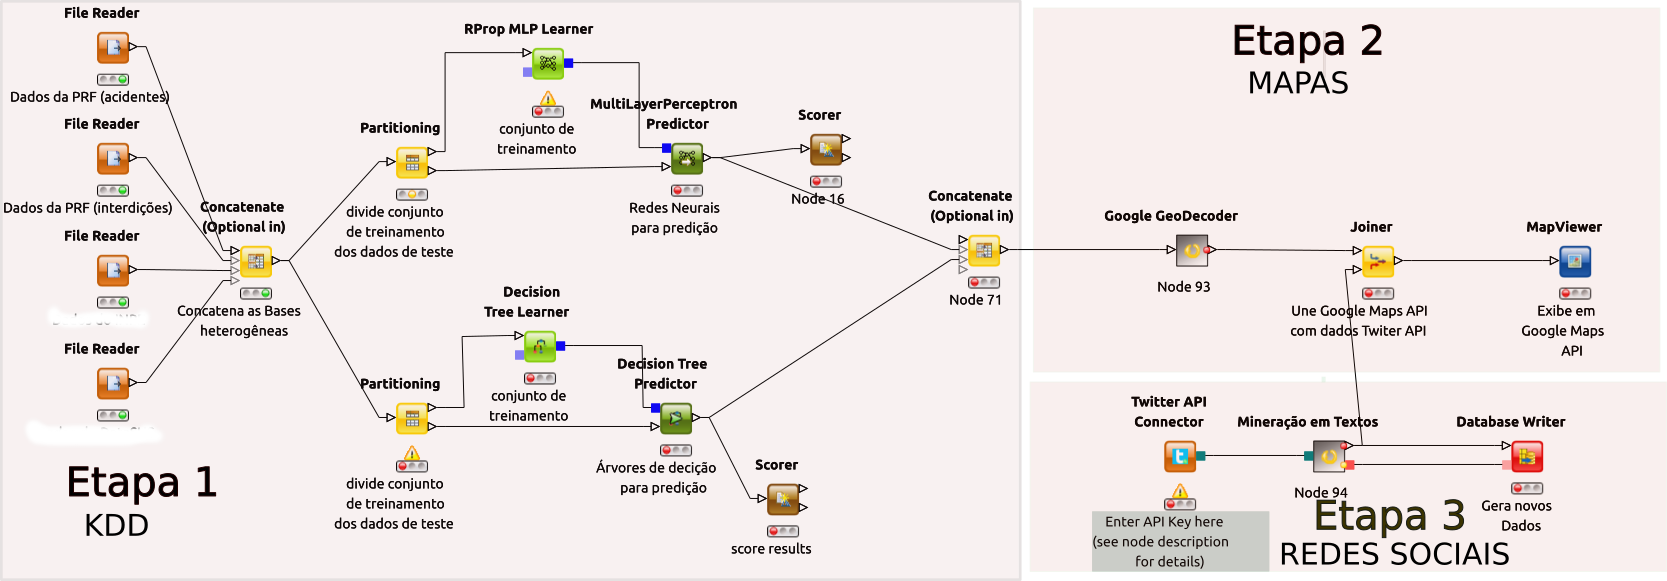
\includegraphics[width=175mm, height=75mm]{Figuras/Cronograma/metodologia.png}\\
\tiny Fonte: autor
\end{figure}

A \textbf{etapa 1} contempla a fases da coleta das bases de dados históricas, preparação dos dados e construção das variáveis do modelo preditivo.
  \begin{enumerate}
    \item O modelo preditivo integra bases de dados, tais como: Polícia Rodoviária Federal -- PRF, Batalhão de Polícia de Transito -- BPRv.
 
    \item Algumas dessas informações também estão disponíveis em base de dados abertas, como sugere o Portal da Transparência, nos servidores da PRF além de outras
	  informações para complementar o sistema estão disponíveis na Internet sendo atualizadas pela PRF através de uma API aberta, esta pode 
	  ser configurável para se ligar ao nosso sistema.
    \item A conclusão dessa etapa ocorre com a Mineração dos dados e a extração de conhecimento.
	  Os ''outputs`` dessa etapa consiste em transformar os dados provenientes da mineração em coordenadas geográficas. 
	  As coordenadas geográficas são agrupadas a priori formando ''cluster`` de dados exibidos em mapas vetoriais.\\
\end{enumerate}
  
A \textbf{segunda} etapa da metodologia contempla:
 \begin{enumerate}
    \item Representação da malha viária em mapas de bases vetoriais;
    \item Um ambiente de simulação interativa que utiliza uma plataforma baseada em API como QGIS e Google Maps.
  \end{enumerate}

A \textbf{terceira} e última etapa consiste em um módulo com as seguintes características:
  \begin{enumerate}
     \item Um módulo dinâmico onde são capturados ``feeds'' de redes sociais, por exemplo pelo Twitter. 
	Essa técnica faz um arco cibernético mantendo o sistema atualizado de informações.
     %\item Através de um interligação a um banco de dados, esses ``feeds'' poderão ser usados para futuras predições.
  \end{enumerate}




\section{A construção do Modelo preditivo}

O modelo preditivo foi construído utilizando bases de dados históricas da PRF (de acidentes e de paralisações ex: protestos) entre Janeiro de 2007 a 
Dezembro 2015. As bases de dados do Batalhão de Polícia de Rodoviária estadual -- BPRv vieram entre Janeiro/2010 a Julho/2016, cortes em ambas as bases foram feitos para adequar as datas até 2015. 
Essas bases de dados são integradas gerando um único e complexo modelo preditivo acoplado a estrutura dinâmica.


\subsection{Aplicação do CRISP-DM}
O CRISP-DM nesta pesquisa ajudou a guiar as
escolhas nos momentos em que os resultados pareciam não
fazer sentido algum, contudo por ser um processo recursivo, o
retorno aos fundamentos dessa metodologia prevê que haja
ajustes necessários a fim de se atingir os objetivos da proposta.

A ideia metodológica proposta para esta pesquisa também
contemplou todas as fases do KDD conforme descrito a seguir.

\subsection{Aplicação das fases da Mineração ao KDD}

Seleção: Nesta etapa foram coletadas as informações
provenientes das bases de dados da Policia Rodoviária Federal
(PRF) de 2007 a 2015, uma vez que nosso interesse era o de
analisar os últimos dez anos, no entanto, como a base de dados
só dispunha de informações a partir de 2007, foram
considerados os nove anos disponíveis. A PRF dispõe em
banco de dados relacionais alguns desses dados na Internet,
contudo no artigo “Uma análise da qualidade dos dados
relativos aos boletins de ocorrências das rodovias federais para
o processo de Mineração de Dados” COSTA, BERNARDINI,
LIMA \cite{Costa2015} destacam a não padronização e não aceitação dos
dados pela comunidade internacional EAVES, D. \cite{Eaves} sugere
que os dados sejam disponibilizados na maneira como foram
coletados. A primeira base de dados coletada diretamente dos
servidores da PRF continha relatório de acidentes e a segunda a
de interdições. A partir dos dados capturados na base da PRF
utilizamos como variáveis de entrada:

\begin{itemize}
 \item Condição da Pista: {Seca, Com burados, Molhada, Em obras, Com material granulado, Oleosa, Enlameada, Com gelo, Outras}
 \item Restrição de visibilidade: {Inexistente, Veículo Estacionado, Poeira/Fumaça/neblina, Vegetação, Ofuscamento, Cartazes/faixas, Placas}
 \item Traçado da via: {Reta, Curva, Cruzamento, Defeito}
 \item Tipo de veículo: {Automóvel, Caminhoneta, Motocicletas, Caminhão, Caminhão-trator, Bicicleta, Caminhonete, Ônibus, Motoneta, Micro-ônibus, Trator
 de rodas, Carroça, Caminhão-Tanque, Semi-Reboque, Utilitário, Ciclomotor, Charrete, Carro-de-mão, Quadriciclo, Trator misto, Reboque, Trator de esteiras,
 Não informado, Não se aplica, Não identificado}
\end{itemize}

Preprocessamento: Nesta fase foram retiradas as variáveis,
sendo consideradas por conterem inconsistência e “missing
data”, como, por exemplo, informações acerca de latitude e
longitude. Cabe destacar que a base, como um todo,
apresentava sérias inconsistências, uma vez que, por exemplo,
um mesmo acidente, quando envolvia dois ou mais veículos,
era lançado na base duas ou mais vezes, em função da
quantidade de veículos envolvidos. Foram eliminadas variáveis
em duplicidade (i.e. as variáveis Mês, Ano que apareciam
separadamente, já aviam sido contempladas na variável Data.).

Transformação: Foram criadas as variáveis “Tipo de
paralisação”, contemplando acidentes sem mortos e com, no
máximo, dois veículos envolvidos; “Dias da semana”
(domingo, segunda-feira,....sábado); “Ajuste de horas” (i.e. 17h58, 17h59, 18h, 18h01, 18h02, arredondadas para 18h);
“Ajuste de Km” (seguiu a mesma lógica do ajuste de horas).

Mineração de dados: O algoritmo escolhido para a pesquisa
foi Árvore de decisão que possibilita uma interpretação
imediata e de fácil compreensão. Como ferramentas, foram
escolhidas o Knime \cite{Knime} e R \cite{R-cran} e o Weka \cite{Weka}, com objetivo
de estabelecer uma comparação entre ambos, cuja intenção era
produzir um classificador mais preciso. Nessa direção, a
técnica Ensamble de classificadores \cite{Bernardini} estabelece que a
combinação de um ou mais classificadores iguais, ou mais de
um classificador diferente, aumenta a precisão. Tanto na
ferramenta Knime com Weka o algoritmo é chamado de J48,
uma vez que se trata da implementação Java do algoritmo
C4.5, no R a biblioteca “rparty” implementa esse algoritmo.
Para escolha das variáveis de input foi calculado a correlação
linear entre todas as variáveis, entre as variáveis BR e
Delegacia (variável que agrega municípios) obteve correlação
linear de 0,653, já entre Tipo de Acidente e Traçado via a
correlação foi baixa, apenas 0,14, variáveis com correlação
linear abaixo disso foram descartadas.

Interpretação/Avaliação: Produção de árvores de decisão a
partir do estabelecimento de diferentes nós-raízes, definidos em
virtude da correlação linear encontrada.

\pagebreak

%++++++++++++++++++++++++++++++++++++++++++++++++++++++++++++++++++++++++++++++++++++++++++++++
\subsection{Dados encontrados antes da Mineração}

A grande maioria dos acidentes ocorre com pista seca, sem restrição de visibilidade. 
A cor vermelha é referente a BR 101, a cor azul à BR 232, seguido das outras menos significativas.

\begin{figure}[h]
	\caption{Hora do acidente (1) --- Concentração em torno da hora (2) }
	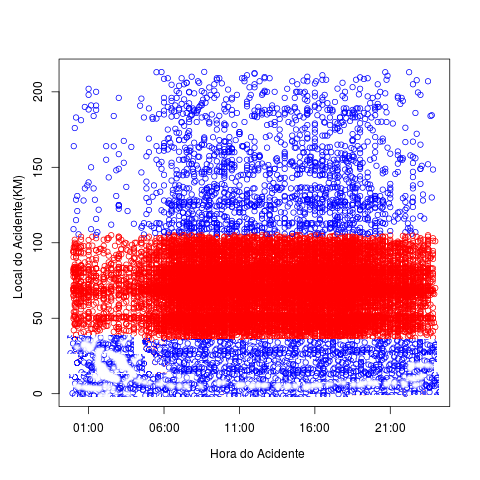
\includegraphics[width=7cm,height=7cm]{Figuras/Preprocess/br101.png}
	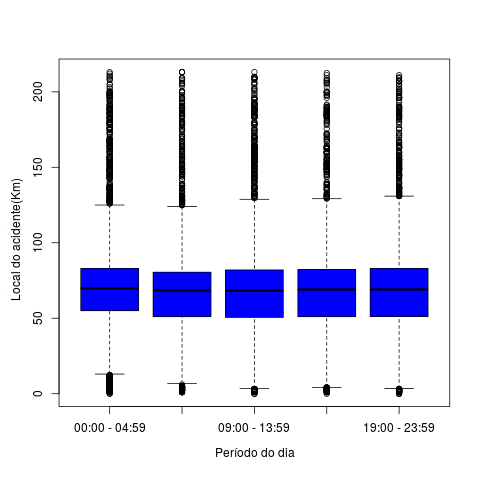
\includegraphics[width=7cm,height=7cm]{Figuras/Preprocess/br101_2.png}
	
\end{figure}

\quad \quad
\begin{figure}[h]
	\centering
	\caption{ Frequência}
	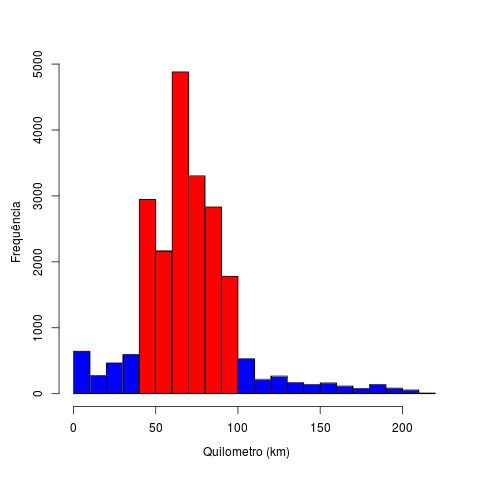
\includegraphics[width=7cm,height=7cm]{Figuras/Preprocess/br101_4.png}
\end{figure}

O gráfico 4.2(1), 4.2(2)  e 4.3 contém dados da BR 101 uma das mais importantes para o nordeste brasileiro pelo seu tráfego intenso. 
A gráfico 4.2(1) representa os acidentes que ocorreram a cada hora (abcissa) em cada Km (ordenada) nos últimos nove anos. 
O  gráfico 4.2(2) corresponde à frequência do local onde ocorreram esses acidentes. 
É possível perceber que há determinados locais, na rodovia, onde se concentram os acidentes. 
O terceiro gráfico, tipo ‘boxplot’, exibe a concentração das ocorrências em torno da mediana dessa localidade (Km). 
Especulou-se a priori que a variável “traçado da rodovia” ou que as condições climáticas poderiam ter influência na causa dos acidentes, contudo mais adiante descobrimos outros condicionantes que influenciam mais fortemente essas ocorrências. 
É possível perceber no gráfico i, que alguns padrões especialmente em determinados locais (Km), por exemplo na BR 101 entre os Km 40 e 100 ocorrem acidentes a partir da 05h da manhã até as 23h. 



\begin{figure}[h]
	\caption{Hora do acidente (1) --- Concentração em torno da hora (2) }
	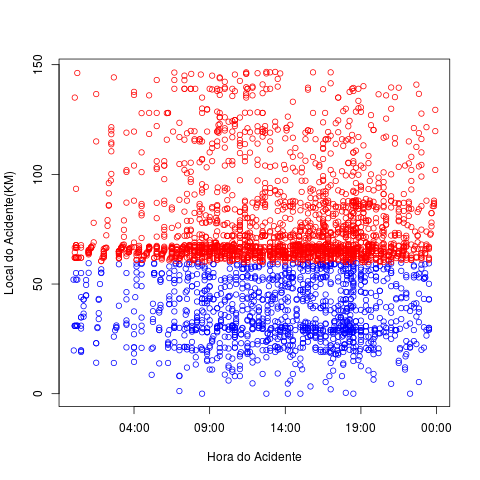
\includegraphics[width=7cm,height=7cm]{Figuras/Preprocess/br104_1.png}
	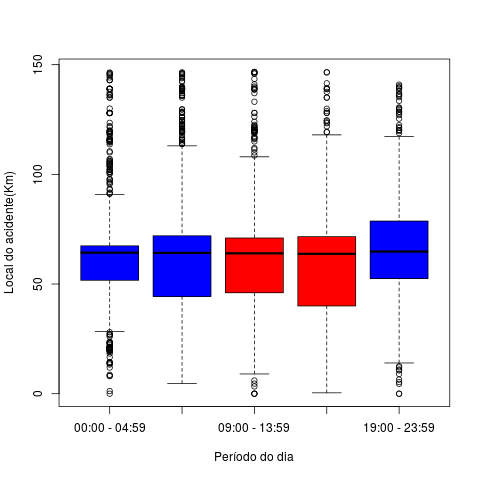
\includegraphics[width=7cm,height=7cm]{Figuras/Preprocess/br104_2.png}

\end{figure}

\quad \quad
\begin{figure}[h]
	\centering
	\caption{ Frequência}
	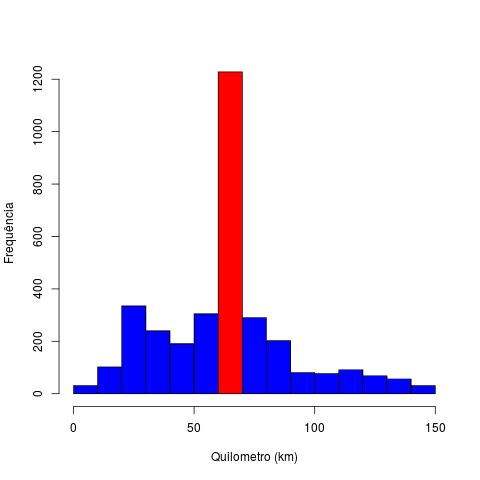
\includegraphics[width=7cm,height=7cm]{Figuras/Preprocess/br104_3.png}
\end{figure}

O gráfico 4.4(1), 4.4(2)  e 4.5 contém dados da BR 104 que atravessa seia municípios de Pernambuco, detre ele Caruaru que apresenta uma das maiores frotas de veículos do interior. 
A gráfico 4.4(1) representa os acidentes que ocorreram a cada hora (abcissa) em cada Km (ordenada) nos últimos nove anos.
O  gráfico 4.4(2) corresponde à frequência do local onde ocorreram esses acidentes. 
É possível perceber que há determinados locais, em torno do Km 60 na rodovia, onde se concentram os acidentes. 
O terceiro gráfico, tipo ‘boxplot’, exibe a concentração das ocorrências em torno da mediana dessa localidade (Km). 
É possível perceber no gráfico i, que alguns padrões especialmente em determinados locais (Km), por exemplo no Km 60 ocorrem acidentes a partir da 04h da manhã até as 23h. 
Destaca-se que esta rodovia atravessa o trecho urbano de Caruaru por onde  passa por dia mais de 50.000 veículos.


\pagebreak
%++++++++++++++++++++++++++++++++++++++++++++++++++++++++++++++++++++++++++++++++++++++++++++++

\begin{figure}[h]
	\caption{Hora do acidente (1) --- Concentração em torno da hora (2) }
	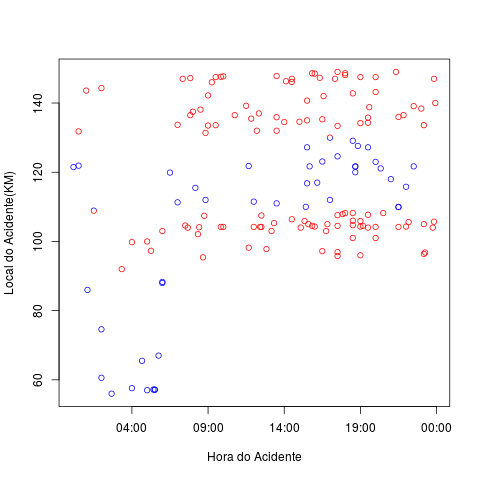
\includegraphics[width=7cm,height=7cm]{Figuras/Preprocess/br110_1.png}
	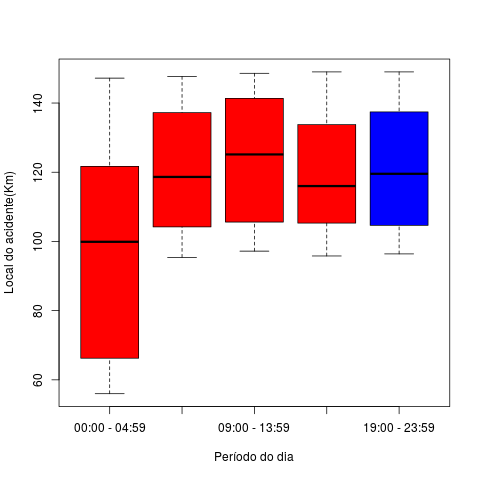
\includegraphics[width=7cm,height=7cm]{Figuras/Preprocess/br110_2.png}

\end{figure}


\quad \quad
\begin{figure}[h]
	\centering
	\caption{ Frequência}
	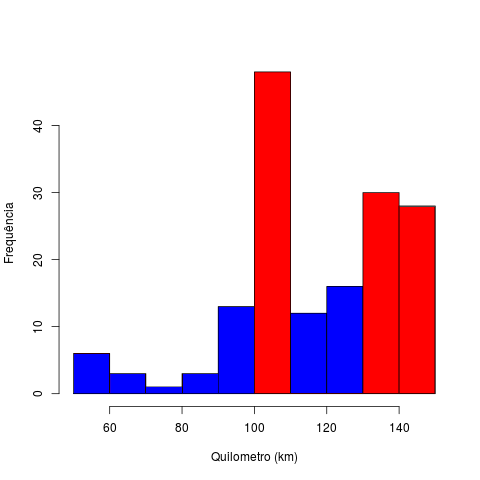
\includegraphics[width=7cm,height=7cm]{Figuras/Preprocess/br110_3.png}
\end{figure}

\pagebreak
%++++++++++++++++++++++++++++++++++++++++++++++++++++++++++++++++++++++++++++++++++++++++++++++

\begin{figure}[h]
	\caption{Hora do acidente (1) --- Concentração em torno da hora (2) }
	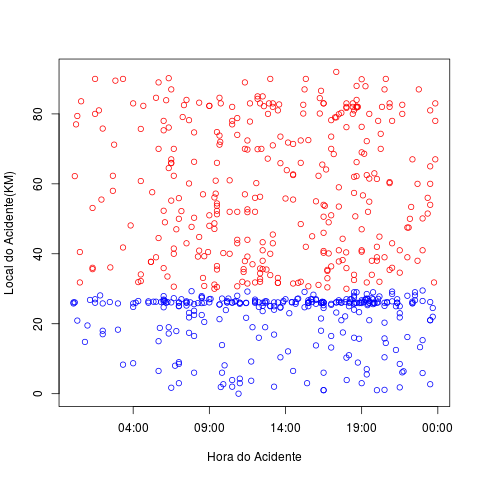
\includegraphics[width=7cm,height=7cm]{Figuras/Preprocess/br116_1.png}
	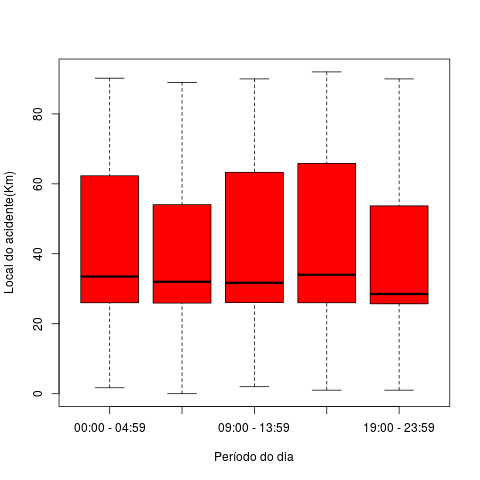
\includegraphics[width=7cm,height=7cm]{Figuras/Preprocess/br116_2.png}

\end{figure}

\quad \quad
\begin{figure}[h]
	\centering
	\caption{ Frequência}
	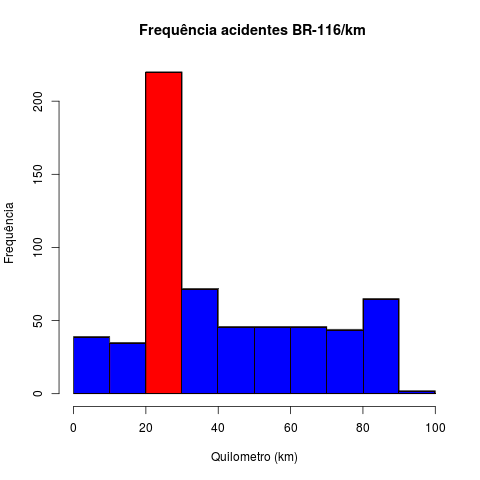
\includegraphics[width=7cm,height=7cm]{Figuras/Preprocess/br116_3.png}
\end{figure}
O gráfico 4.8(1), 4.8(2)  e 4.9 contém dados da BR 116 uma das mais importantes para o nordeste brasileiro e do paíspelo seu tráfego intenso, atravessa o país inteiro, desde o Rio Grande do Sul até o Ceará. 
A gráfico 4.8(1) representa os acidentes que ocorreram a cada hora (abcissa) em cada Km (ordenada) nos últimos nove anos. 
O  gráfico 4.8(2) corresponde à frequência do local onde ocorreram esses acidentes. 
É possível perceber que há determinados locais, na rodovia, onde se concentram os acidentes. 
O terceiro gráfico, tipo ‘boxplot’, exibe a concentração das ocorrências em torno da mediana dessa localidade (Km). 
Especulou-se a priori que a variável “traçado da rodovia” ou que as condições climáticas poderiam ter influência na causa dos acidentes, contudo mais adiante descobrimos outros condicionantes que influenciam mais fortemente essas ocorrências. 
É possível perceber no gráfico 4.9, que alguns padrões especialmente em determinados locais (Km), por exemplo, há um padrão nos acidentes nos Km 30 onde ocorrem acidentes a partir da 04h da manhã até as 22h. 

\pagebreak
%++++++++++++++++++++++++++++++++++++++++++++++++++++++++++++++++++++++++++++++++++++++++++++++

\begin{figure}[h]
	\caption{Hora do acidente (1) --- Concentração em torno da hora (2)}
	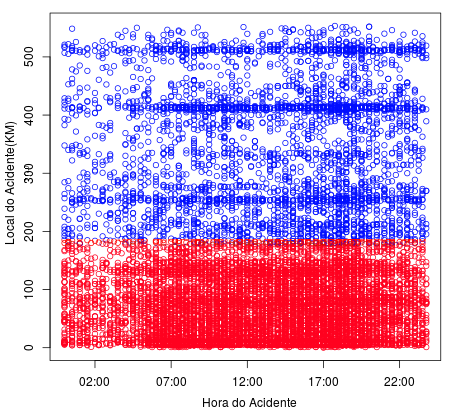
\includegraphics[width=7cm,height=7cm]{Figuras/Preprocess/br232_1.png}
	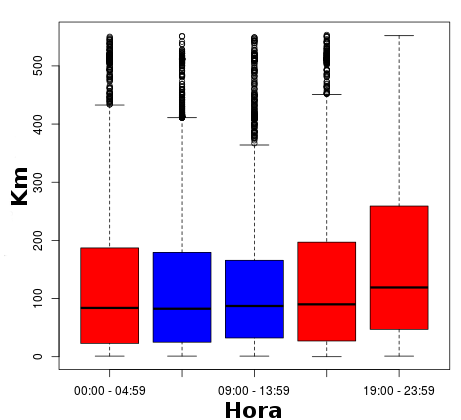
\includegraphics[width=7cm,height=7cm]{Figuras/Preprocess/br232_2.png}

\end{figure}

\quad \quad
\begin{figure}[h]
	\centering
	\caption{ Frequência}
	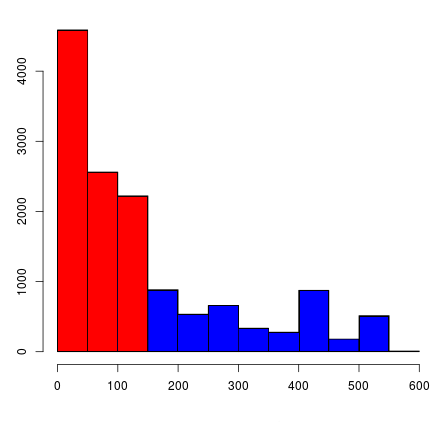
\includegraphics[width=7cm,height=7cm]{Figuras/Preprocess/br232_3.png}
\end{figure}

O gráfico 4.10(1), 4.10(2)  e 4.11 contém dados da BR 101 uma das mais importantes para o nordeste brasileiro pelo seu tráfego intenso. 
A gráfico 4.10(1) representa os acidentes que ocorreram a cada hora (abcissa) em cada Km (ordenada) nos últimos nove anos. 
O  gráfico 4.10(2) corresponde à frequência do local onde ocorreram esses acidentes. 
É possível perceber que há determinados locais, na rodovia, onde se concentram os acidentes. 
O terceiro gráfico, tipo ‘boxplot’, exibe a concentração das ocorrências em torno da mediana dessa localidade (Km). 
Especulou-se a priori que a variável “traçado da rodovia” ou que as condições climáticas poderiam ter influência na causa dos acidentes, contudo mais adiante descobrimos outros condicionantes que influenciam mais fortemente essas ocorrências. 
É possível perceber no gráfico 4.11, que alguns padrões especialmente em determinados locais (Km), por exemplo, na BR 232 há um padrão nos acidentes nos Km 0, 90, 110, 260, 410 e
500. ocorrem acidentes a partir da 00h da manhã até as 23h. 


\pagebreak
%++++++++++++++++++++++++++++++++++++++++++++++++++++++++++++++++++++++++++++++++++++++++++++++

\begin{figure}[h]
	\caption{Hora do acidente (1) --- Concentração em torno da hora (2)}
	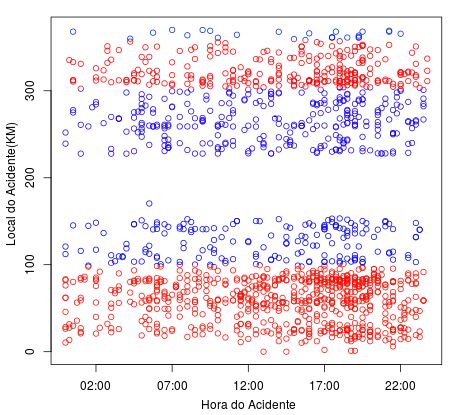
\includegraphics[width=7cm,height=7cm]{Figuras/Preprocess/br316_1.png}
	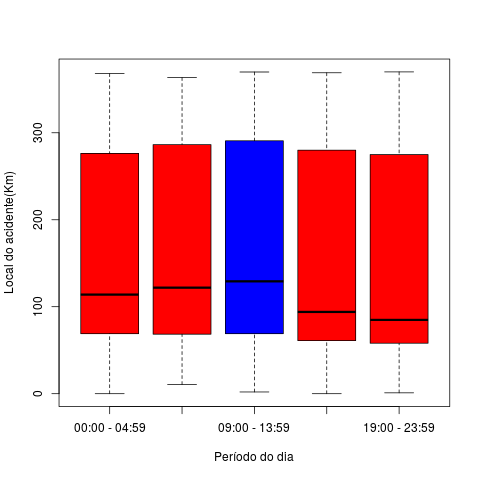
\includegraphics[width=7cm,height=7cm]{Figuras/Preprocess/br316_2.png}

\end{figure}

\quad \quad
\begin{figure}[h]
	\centering
	\caption{ Frequência}
	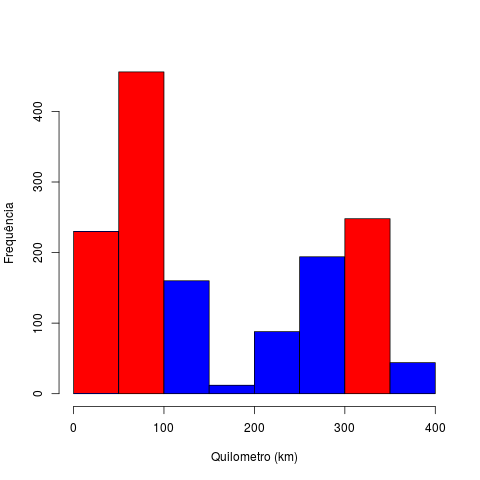
\includegraphics[width=7cm,height=7cm]{Figuras/Preprocess/br316_3.png}
\end{figure}


\pagebreak
%++++++++++++++++++++++++++++++++++++++++++++++++++++++++++++++++++++++++++++++++++++++++++++++

\begin{figure}[h]
	\caption{Hora do acidente (1) --- Concentração em torno da hora (2)}
	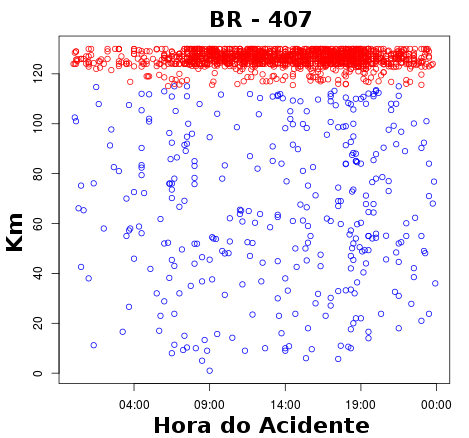
\includegraphics[width=7cm,height=7cm]{Figuras/Preprocess/br407_1.png}
	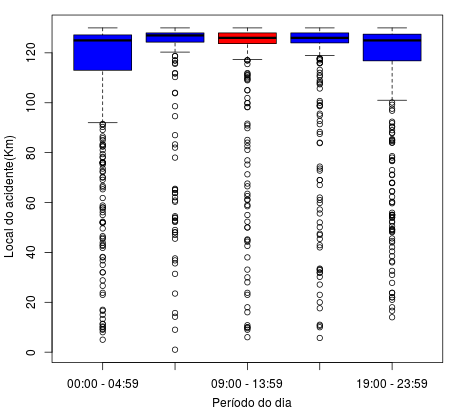
\includegraphics[width=7cm,height=7cm]{Figuras/Preprocess/br407_3.png}

\end{figure}

\quad
\begin{figure}[h]
	\centering
	\caption{ Frequência}
	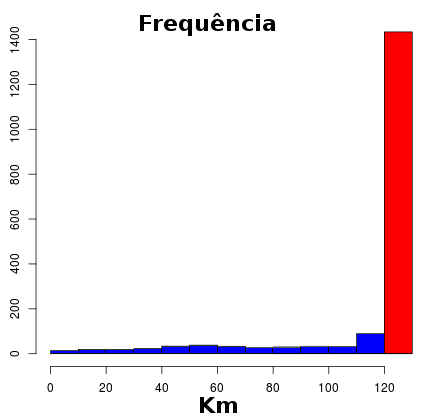
\includegraphics[width=7cm,height=7cm]{Figuras/Preprocess/br407_2.png}
\end{figure}

Na BR 407 os acidentes se concentram na altura do Km
130.


%++++++++++++++++++++++++++++++++++++++++++++++++++++++++++++++++++++++++++++++++++++++++++++++

\begin{figure}[h]
	\caption{Hora do acidente (1) --- Concentração em torno da hora (2)}
	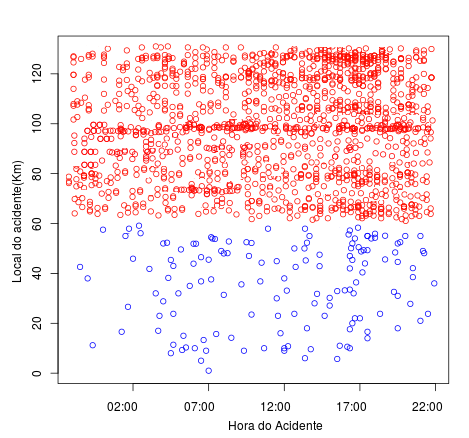
\includegraphics[width=7cm,height=7cm]{Figuras/Preprocess/br408_1.png}
	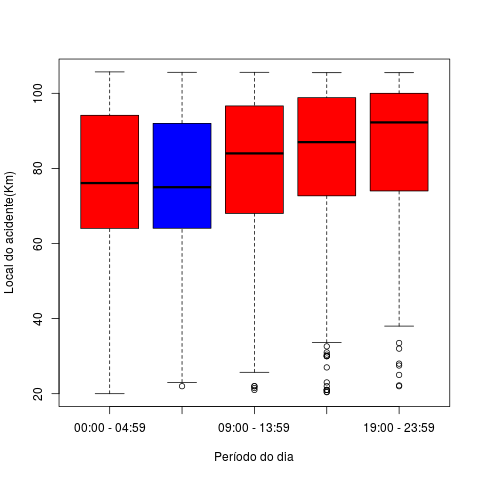
\includegraphics[width=7cm,height=7cm]{Figuras/Preprocess/br408_2.png}

\end{figure}

\quad \quad
\begin{figure}[h]
	\centering
	\caption{ Frequência}
	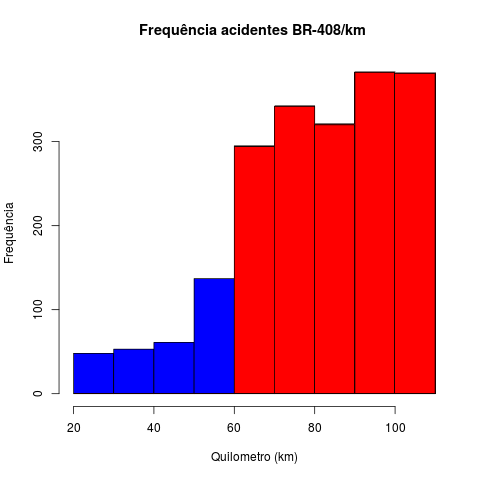
\includegraphics[width=7cm,height=7cm]{Figuras/Preprocess/br408_3.png}
\end{figure}


\pagebreak
%++++++++++++++++++++++++++++++++++++++++++++++++++++++++++++++++++++++++++++++++++++++++++++++

\begin{figure}[h]
	\caption{Hora do acidente (1) --- Concentração em torno da hora (2)}
	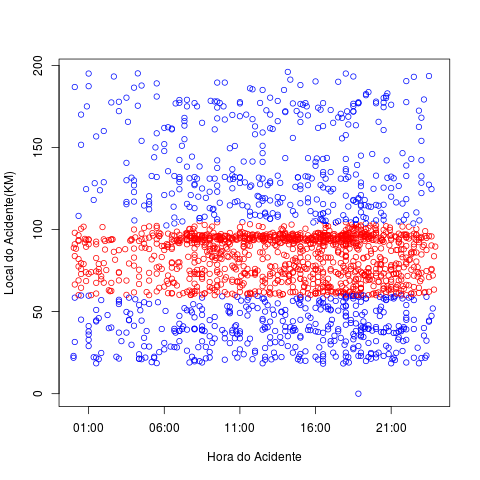
\includegraphics[width=7cm,height=7cm]{Figuras/Preprocess/br423_1.png}
	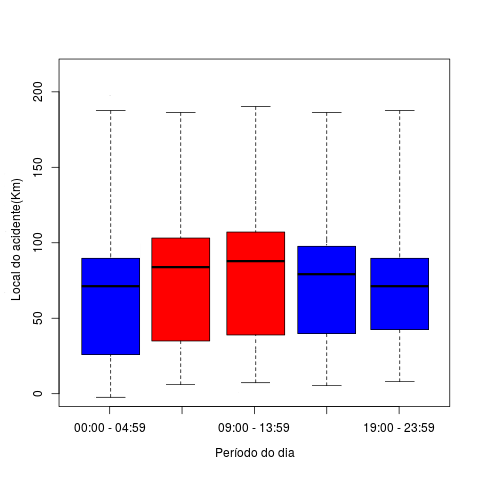
\includegraphics[width=7cm,height=7cm]{Figuras/Preprocess/br423_2.png}
	
\end{figure}

\quad \quad
\begin{figure}[h]
	\centering
	\caption{ Frequência}
%	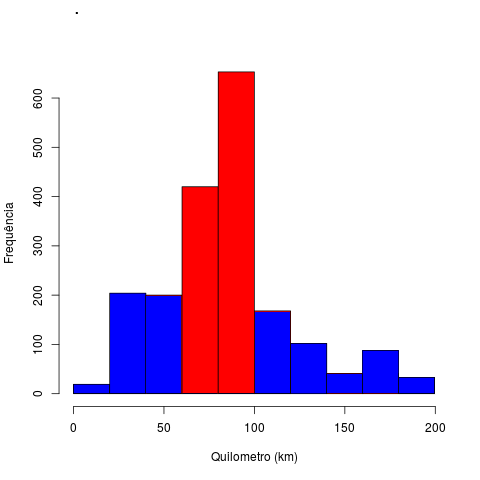
\includegraphics[width=5cm,height=6cm]{Figuras/Preprocess/br423_3.png}
\end{figure}


\pagebreak
%++++++++++++++++++++++++++++++++++++++++++++++++++++++++++++++++++++++++++++++++++++++++++++++

\begin{figure}[h]
	\caption{Hora do acidente (1) --- Concentração em torno da hora (2)}
	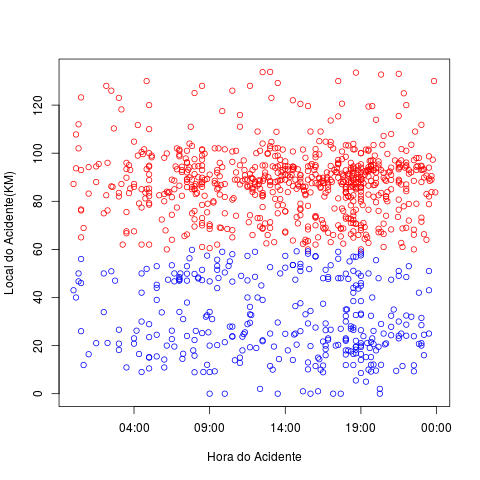
\includegraphics[width=7cm,height=7cm]{Figuras/Preprocess/br424_1.png}
	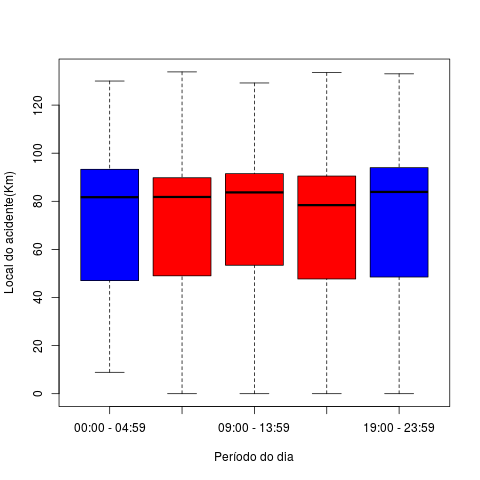
\includegraphics[width=7cm,height=7cm]{Figuras/Preprocess/br424_2.png}
	
\end{figure}

\quad \quad
\begin{figure}[h]
	\centering
	\caption{ Frequência}
	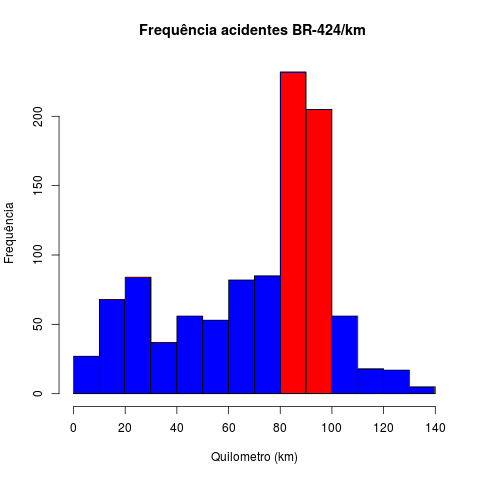
\includegraphics[width=7cm,height=7cm]{Figuras/Preprocess/br424_3.png}
\end{figure}


\pagebreak
%++++++++++++++++++++++++++++++++++++++++++++++++++++++++++++++++++++++++++++++++++++++++++++++


\begin{figure}[h]
	\caption{Hora do acidente (1) --- Concentração em torno da hora (2)}
	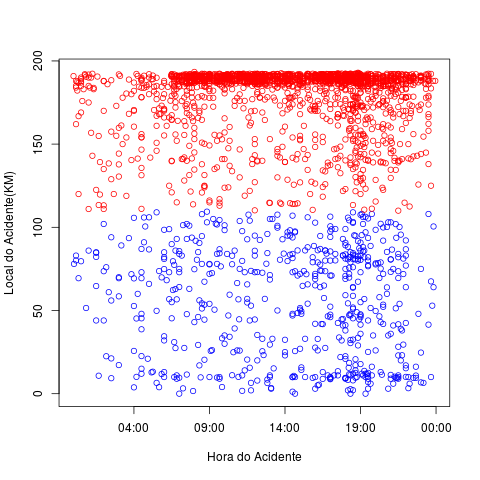
\includegraphics[width=7cm,height=7cm]{Figuras/Preprocess/br428_1.png}
	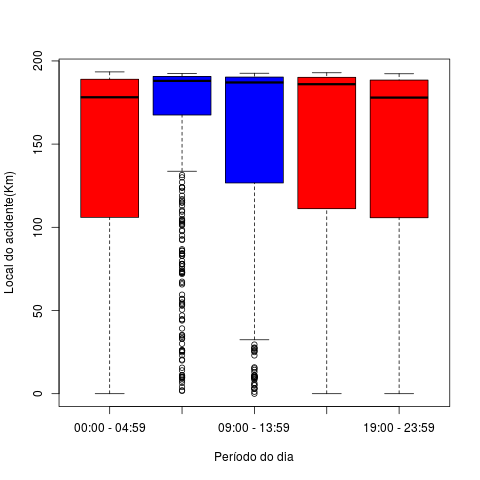
\includegraphics[width=7cm,height=7cm]{Figuras/Preprocess/br428_2.png}
	
\end{figure}

\quad \quad
\begin{figure}[h]
	\centering
	\caption{ Frequência}
	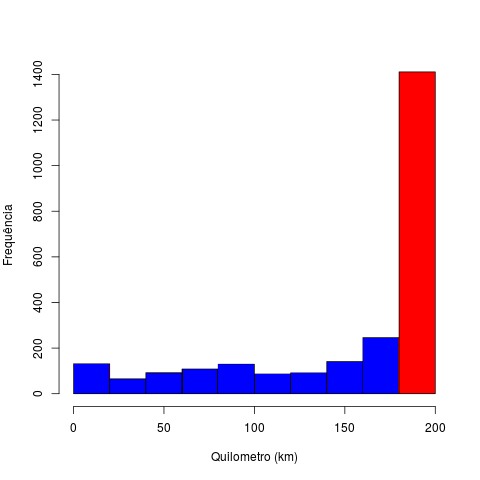
\includegraphics[width=7cm,height=7cm]{Figuras/Preprocess/br428_3.png}
\end{figure}


\pagebreak
%++++++++++++++++++++++++++++++++++++++++++++++++++++++++++++++++++++++++++++++++++++++++++++++

\begin{figure}[ht]
\begin{center}
\caption{Tipo de Veículo X Num. Acidentes}
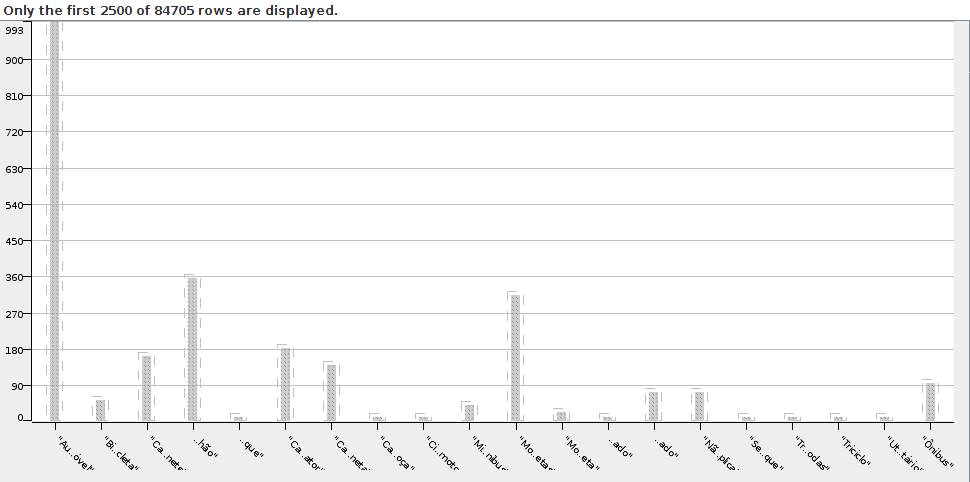
\includegraphics[width=150mm, height=80mm]{Figuras/Preprocess/TipoVeiculoXNumAciden.png}\\
\tiny Fonte: autor
\end{center}
\end{figure}

O maior número de acidentes ocorre com Automóvel de passeio, provavelmente condutores comuns, não profissionalizados.
O Caminhão é o segundo veículo que mais se envolve em acidentes, seguido das motonetas. 
Esses dados são referentes ao período entre 2007 à 2015.

\begin{figure}[ht]
\begin{center}
\caption{Traçado da via X Num. Acidentes}
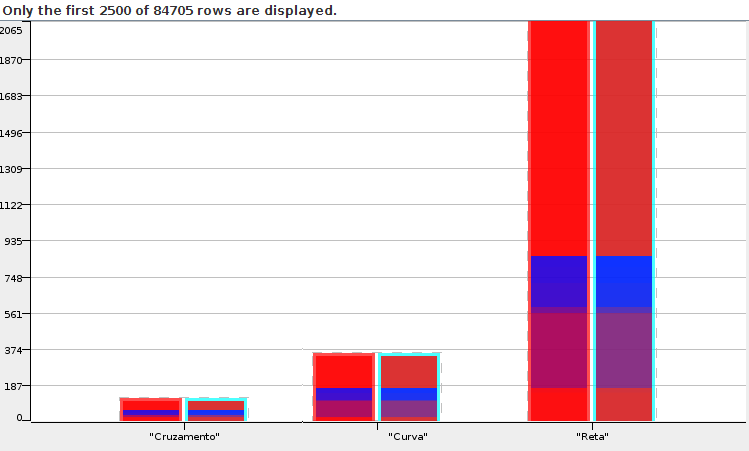
\includegraphics[width=120mm, height=70mm]{Figuras/Preprocess/TracadoViaNumAcident.png}\\
\tiny Fonte: autor
\end{center}
\end{figure}

O tipo de traçado da via não influência nas estatísticos de acidenes, pois a grande maioria dos acidentes ocorre em linha reta.
Esse comportamento do condutor nos faz crer o condutor é o responsável pelo maior número de ocorrências nas BRs.
Isso direciona nossa pesquisa para analisar e antever o comportamento do condutor, as condições da rodovia e ambientais nessa base
de dados não são fatores relevantes.

\pagebreak



\subsection{Dados encontrados após a Mineração}

Os resultados da classificação encontrados estão contidos a
seguir, dentre os classificadores disponíveis no Weka os que
melhor apresentaram resultados foram: o Naive Bayes e a
Árvore de Decisão
As variáveis “Tipo de Acidente”, “Gravidade” e
“BRajustada” foram escolhidas pelas características de ganho
de informação dado pelo cálculo da entropia. “BRajustada”
significa ... A literatura aconselha que os nós da raiz dos
classificadores, em especial Árvores de decisão, tenham maior
entropia, como a variável “Tipo de Acidente”, no entanto o
grande número de ramificações que esta variável gerou não foi
interessante para o objetivo da pesquisa; explicar o porquê das
causas dos acidentes (pontos fortemente destacados nos gráficos com rótulo (1)). 
A seguir apresenta-se a nomenclatura da acurácia encontrada na classificação.

\begin{itemize}
	\item TP: True Positive;
	\item FP: False Positive;
	\item Prec.: Precison = TP/(TP +FP);
	\item Recall = TP/ (TP + FN);
	\item F-Me: F-measure ou f-score = 2 * Precison * Recall / (Precision + Recall);
	\item AUC: Area Under Curve (Roc);
\end{itemize}
    
\subsection{Métrica dos classificadores}

\begin{enumerate}
	\item[(i)] Variável: Tipo de Acidente (Entropia: 3.0686)
		\begin{table}[!ht]
			\centering
			%\caption{Volume de dados no mundo}
			\vspace{1mm}
			\begin{tabular}{l|c|c}
				\hline
				\textbf{Descrição} & \textbf{Valores} & \textbf{Percentual} \\
				\hline
				Instâncias Corretamente Classificadas & 7987 & 47.6324\% \\
				Instâncias Incorretamente Classificadas & 8781 & 52.3676\% \\
				Erro médio absoluto & 0.0786 & ---  \\
				Erro médio quadratico & 0.2083 & --- \\
			\end{tabular}
		\end{table}
		
		\pagebreak
		
		\begin{table}[!ht]
			\centering
			\caption{Detalhe da acurácia para classe Tipo Acidente}
			\vspace{1mm}
			\begin{tabular}{l|c|c|c|c|c|l}
				\hline
				\textbf{TP} & \textbf{FP} & \textbf{Prec.} & \textbf{Recall} & \textbf{F-Me.} & \textbf{AUC} & \textbf{Classe} \\
				\hline
				0.337 & 0.059 & 0.372 & 0.337 & 0.354 & 0.738 & Colisão transversal \\
				0.026 & 0.012 & 0.066 & 0.026 & 0.038 & 0.684 & Colisão com objeto fixo \\
				0.925 &	0.003 &	0.920 & 0.925 & 0.923 & 0.980 & Atropelamento de pessoa \\
				0.463 &	0.157 &	0.448 &	0.463 &	0.455 &	0.731 &	Colisão lateral \\
				0.682 &	0.259 & 0.545 & 0.682 & 0.606 & 0.773 & Colisão traseira \\
				0.485 & 0.024 & 0.409 & 0.485 & 0.443 & 0.893 & Queda de Moto/bicicleta \\
				0.322 & 0.002 & 0.528 & 0.322 & 0.400 & 0.744 & Colisão com bicicleta \\
				0.122 & 0.026 & 0.229 & 0.122 & 0.159 & 0.786 & Capotamento \\
				0.890 & 0.014 & 0.655 & 0.890 & 0.755 & 0.954 & Atropelamento de animal \\
				0.048 & 0.007 & 0.243 & 0.048 & 0.081 & 0.729 & Colisão frontal \\
				0.440 & 0.089 & 0.366 & 0.440 & 0.399 & 0.792 & Saída de Pista \\
				0.000 & 0.000 & 0.000 & 0.000 & 0.000 & 0.658 & Colisão c/ objeto móvel\\
				0.096 & 0.006 & 0.292 & 0.096 & 0.144 & 0.774 & Tombamento \\
				0.000 & 0.000 & 0.000 & 0.000 & 0.000 & 0.616 & Derramamento de Carga \\
				0.041 & 0.000 & 0.400 & 0.041 & 0.074 & 0.627 & Danos Eventuais \\
				0.000 & 0.000 & 0.000 & 0.000 & 0.000 & 0.733 & Incêndio \\	
			\end{tabular}
		\end{table}
		
		\begin{table}[!ht]
			\centering
			\caption{Matriz de confusão para a variável Tipo de acidente}
			\vspace{1mm}
			\begin{tabular}{l|c|c|c|c|c|c|c|l}
				\hline
				\textbf{a} & \textbf{b} & \textbf{c} & \textbf{d} & \textbf{e} & \textbf{f} & \textbf{g} & \textbf{h} & \textbf{Classificadores}\\
				\hline
				527 & 7 & 2 & 385 & 483 & 46 & 2 & 24 & Colisão transversal \\
				16 & 14 & 0 & 69 & 154 & 15 & 0 & 47 & Colisão com objeto fixo \\
				8 & 0 & 483 & 16 & 14 & 0 & 0 & 0 & Atropelamento de pessoa \\
				336 & 30 & 8 & 1674 & 1217 & 102 & 8 & 48 & Colisão lateral \\
				250 & 51 & 9 & 835 & 3573 & 105 & 11 & 59 & Colisão traseira \\
				44 & 4 & 1 & 74 & 120 & 266 & 2 & 0 & Queda de Moto/bicicleta \\
				8 & 0 & 0 & 22 & 38 & 3 & 38 & 1 & Colisão com bicicleta \\
				28 & 34 & 5 & 85 & 236 & 1 & 2 & 120 & Capotamento \\
				-- & -- & -- & -- & -- & -- & -- & -- & -- \\	
			\end{tabular}
		\end{table}
		
		Os valores restantes foram omitidos por não representar uma amostra
		adequada, pois..... As variáveis de classe são as mesmas da tabela
		anterior. \\
					
%	\pagebreak	
	\item[(ii)] Variável: Gravidade (Entropia: 0,9997)
	\begin{table}[!ht]
		\centering
		%\caption{Volume de dados no mundo}
		\vspace{1mm}
		\begin{tabular}{l|c|c}
			\hline
			\textbf{Descrição} & \textbf{Valores} & \textbf{Percentual} \\
			\hline
			Instâncias Corretamente Classificadas & 12110 & 72.2209\% \\
			Instâncias Incorretamente Classificadas & 4658 & 27.7791\% \\
			Erro médio absoluto & 0.3816 & ---  \\
			Erro médio quadratico & 0.4368 & --- \\
		\end{tabular}
	\end{table}
	
\pagebreak	
	
	\begin{table}[!ht]
		\centering
		\caption{Detalhe da acurácia para classe Gravidade}
		\vspace{1mm}
		\begin{tabular}{l|c|c|c|c|c|l}
			\hline
			\textbf{TP} & \textbf{FP} & \textbf{Prec.} & \textbf{Recall} & \textbf{F-Me.} & \textbf{AUC} & \textbf{Classe} \\
			\hline
			0.907 & 0.608 & 0.727 & 0.907 & 0.807 & 0.721 & S \\
			0.392 & 0.093 & 0.703 & 0.392 & 0.504 & 0.721 & N \\
				
		\end{tabular}
	\end{table}
	
	\begin{table}[!ht]
		\centering
		\caption{Matriz de confusão para a variável Gravidade}
		\vspace{1mm}
		\begin{tabular}{l|c|l}
			\hline
			\textbf{a} & \textbf{b} & \textbf{Classificadores}\\
			\hline
			9747 & 996 & a = S \\
			3662 & 2363 & b = N \\
		\end{tabular}
	\end{table}
	
	
	\item[(iii)] Variável: BRajustada (Entropia: 2,4128)
	\begin{table}[!ht]
		\centering
		%\caption{Volume de dados no mundo}
		\vspace{1mm}
		\begin{tabular}{l|c|c}
			\hline
			\textbf{Descrição} & \textbf{Valores} & \textbf{Percentual} \\
			\hline
			Instâncias Corretamente Classificadas & 13507 & 80.5522\% \\
			Instâncias Incorretamente Classificadas & 3261 & 19.4478\% \\
			Erro médio absoluto & 0.0469 & ---  \\
			Erro médio quadratico & 0.1656 & --- \\
		\end{tabular}
	\end{table}
	
	\begin{table}[!ht]
		\centering
		\caption{Detalhe da acurácia para classe BR}
		\vspace{1mm}
		\begin{tabular}{l|c|c|c|c|c|l}
			\hline
			\textbf{TP} & \textbf{FP} & \textbf{Prec.} & \textbf{Recall} & \textbf{F-Me.} & \textbf{AUC} & \textbf{Classe} \\
			\hline
			0.902 & 0.178 & 0.812 & 0.902 & 0.854 & 0.917 & BR101 \\
			0.873 & 0.003 & 0.957 & 0.873 & 0.913 & 0.992 & BR104 \\
			0.213 & 0.001 & 0.357 & 0.213 & 0.267 & 0.816 & BR110 \\
			0.457 & 0.003 & 0.669 & 0.457 & 0.543 & 0.961 & BR116 \\
			0.760 & 0.068 & 0.787 & 0.760 & 0.774 & 0.919 & BR232 \\
			0.893 & 0.006 & 0.800 & 0.893 & 0.844 & 0.985 & BR316 \\
			0.951 & 0.007 & 0.857 & 0.951 & 0.901 & 0.995 & BR428 \\
			0.761 & 0.012 & 0.693 & 0.761 & 0.725 & 0.974 & BR423 \\
			0.461 &	0.006 &	0.599 & 0.461 &	0.521 & 0.957 & BR424 \\
			0.814 & 0.001 & 0.961 & 0.814 & 0.881 & 0.999 & BR407 \\
			0.158 & 0.010 & 0.460 & 0.158 & 0.235 & 0.781 & BR408 \\
		\end{tabular}
	\end{table}
	
	\begin{table}[!ht]
		\centering
		\caption{Matriz de confusão para a variável BRajustada}
		\vspace{1mm}
		\begin{tabular}{l|c|c|c|c|c|c|c|l}
			\hline
			\textbf{a} & \textbf{b} & \textbf{c} & \textbf{d} & \textbf{e} & \textbf{f} & \textbf{g} & \textbf{h} & \textbf{Classificadores}\\
			\hline
			6960 & 0 & 0 & 625 & 0 & 0 & 0 & 0 & BR101 \\
			0 & 1071 & 0 & 156 & 0 & 0 & 0 & 0  & BR104 \\
			0 & 0 & 0 & 625 & 0 & 0 & 26 & 11  & BR110 \\
			0 & 0 & 85 & 0 & 90 & 11 & 0 & 0  & BR116 \\
			970 & 9 & 0 & 3185 & 1 & 0 & 1 & 0  & BR232 \\
			0 & 0 & 27 & 11 & 377 & 7 & 0 & 0  & BR316 \\
			0 & 0 & 0 & 0 & 0 & 95 & 0 & 0  & BR407 \\
			643 & 0 & 0 & 66 & 0 & 0 & 0 & 0  & BR408 \\
			0 & 39 & 0 & 0 & 0 & 0 & 449 & 92  & BR423 \\
			0 & 0 & 0 & 625 & 0 & 0 & 172 & 154  & BR424 \\
			0 & 0 & 15 & 0 & 3 & 675 & 0 & 0  & BR428 \\			
		\end{tabular}
	\end{table}	

\end{enumerate}

A área sob a curva Roc, AUC (Area Under Curve) mede a
relação de verdadeiros positivos contra os falsos positivos,
quanto maior a área da curva ou tanto melhor será o
classificador. Portanto um número de verdadeiros positivos
acima de 80\% e o número de falsos positivos próximo a 0\%
traduzem uma área da curva ROC (AUC) que dão maior confiabilidade
aos testes.

A variável “BRajustada” não teve o maior coeficiente de
entropia encontrado, contudo esta variável apresentou
índices de classificação das instâncias correta acima dos 80\% e
o menor índice de classificação incorreta dentre os dois
classificadores utilizados. Esta variável foi a escolhida para
encabeçar os algoritmos para os resultados encontrados. 

A árvore construída pelo Knime para a mesma variável “Causa do Acidente” => velocidade incompatível está na
próxima figura.
\begin{figure}
\centering
\caption{Árvore de Decisão gerada pelo Knime}
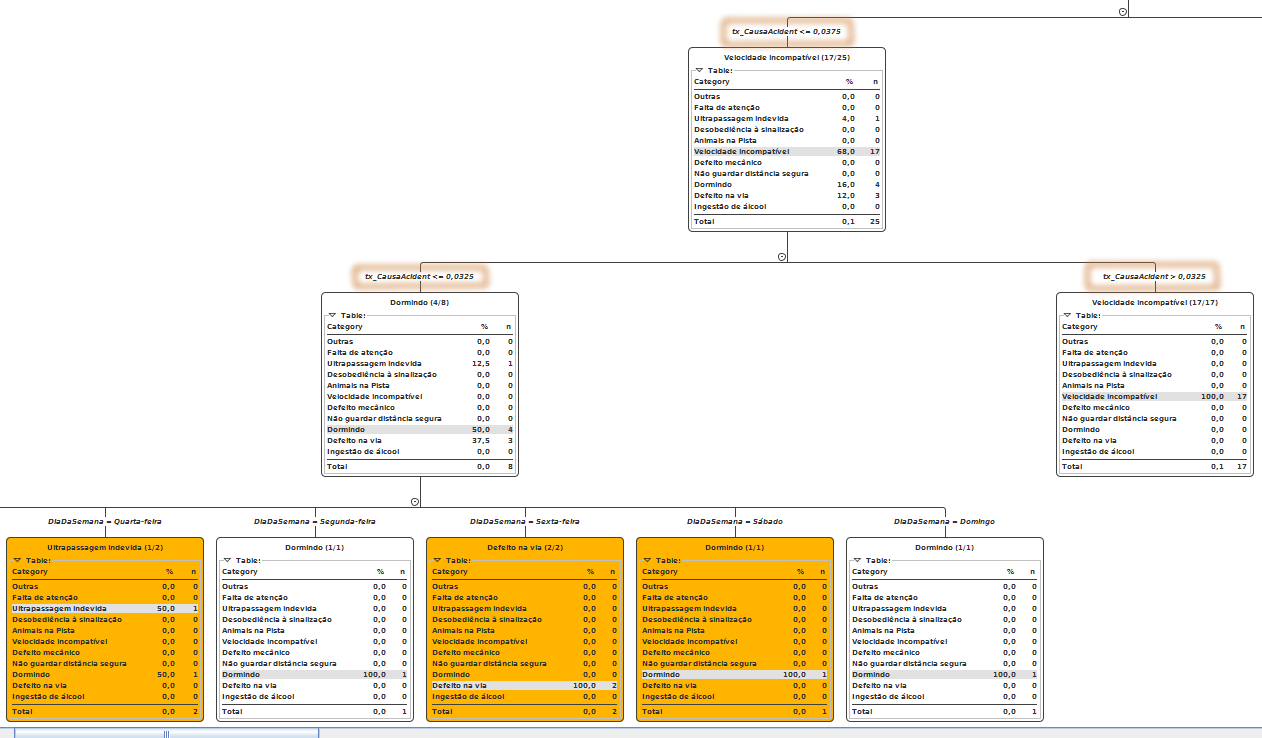
\includegraphics[width=0.7\linewidth]{Figuras/Metodologia/arvoreKnime.png}
\caption{}
\label{fig:arvoreKnime}
\end{figure}


\pagebreak

Também para exemplificar, o nó folha classificou, que nas
quartas-feiras a causa “ultrapassagem indevida”; sextas-feiras:
“defeito na via”; e, caso seja um sábado, a causa é “dormindo”.
Contudo os melhores resultados de acordo com mais alta
precisão segundo a métrica dos classificadores foi a variável
“BRajustada” com curva ROC acima dos 90% em quase todos
as classes, inclusive o classificador Naive Bayes obteve um
desempenho semelhante as Arvores de decisão com essa
variável, somente na BR 408 e BR110 ficou abaixo, o que
confirma os valores encontrados pelo Weka.
Os valores das regras encontradas pelo algoritmo para a
variável “Delegacia” foram:

(a) “Delegacia” [1101(Região Metropolitana)], [BR 101],
[KM: 4], [Traçado da via: Reta], [Gravidade = S (acidente com
mortes) = 
[Causa Acidente: Falta atenção]
[Causa Acidente: Velocidade incompatível]
[Causa Acidente: Ultrapassagem indevida]
[Causa Acidente: Defeito mecânico]
[Causa Acidente: Não guardar distância]
[Causa Acidente: Dormindo]
[Causa Acidente: Ingestão de álcool]

(b) “Delegacia” [1101(Região Metropolitana)], [BR 232],
[KM: 17], [Condição pista: Seca], [Tipo Auto: automóvel]=
[Causa Acidente: Velocidade incompatível]
[Causa Acidente: Ultrapassagem indevida]
[Causa Acidente: Desobediência à sinalização]
[Causa Acidente: Não guardar distância]
[Causa Acidente: Dormindo]
[Causa Acidente: Ingestão de álcool]

Essa variedade de causas explica que o condutor dessa
região não respeita as leis de transito, pode se dizer que e
indisciplinado, pois todos os tipos de causa foram encontrados.
Caso se considere um raio de 50 Km no entorno da capital Recife pode-se dizer que os motoristas tem a mesma
característica, pelo tipo de acidente que acomete nessa área.
Os valores das regras encontradas pelo algoritmo para a
variável “Tipo do Acidente” foram:
(a) “Tipo de Acidente” [região metropolitana]: [Atropelamento
de pessoa], [pista seca], [período: noite], [Br < 116 (101, 104)]
, [Dia da semana: terça-feira]:
[Gravidade = N (sem morte)], [Km <= 69] => falta de atenção.
[Gravidade = S (com morte)] => outras.

Tipo de Acidente: [Atropelamento de pessoa], [pista seca],
[período: noite], [Br < 116 (101, 104)] , [Dia da semana: sexta-
feira]:
[Gravidade = N (sem morte)], [Km <= 58] => falta de atenção.
[Gravidade = S (com morte)] => [Km > 58] [Km <= 67] =>
falta de atenção.

A fata de atenção foi condição “sine qua non”
ocorreram acidentes na região metropolitana do Recife. Para a região no entrono da BR 116 os acidentes com
mortes [Gravidade = S] na quinta-feira o curioso foi que quase
todos os tipos de veículos se envolveram nesse tipo
ocorrências.
Os valores das regras encontradas pelo algoritmo para a
variável “Causa do Acidente” foram:
[Ingestão de álcool], [Tipo de auto: não identificado], [Período:
Manhã] o tipo de acidente => colisão traseira.
[Ingestão de álcool], [Tipo de auto: automóvel], [Traçado da
via: Reta], [Condição da pista: molhada], [Dia da semana]:
[Segunda-feira] => colisão frontal
[Terça-feira] => colisão transversal
[Quarta-feira] => colisão transversal
[Quinta-feira] => saída de pista
[Sexta-feira] => colisão traseira
[Sábado]: [BR = 232] => colisão traseira
	[BR > 232] => colisão frontal

\section{Acoplamento com a estrutura dinâmica}

As predições feitas na primeira fase têm como ``output'' coordenadas geográficas do tipo latitude e longitude.

A estrutura dinâmica é composta por duas API's, uma disponibilizada pela Google, através do Google Maps que está atualmente na versão V3 e 
outra uma API do Twitter. A API do Google Maps proporciona uma ``leitura'' atualizada em forma de mapa no momento em que a estrutura dinâmica ``roda''.

A API do Twitter possibilita atualizar o utilizador de informações recentes, pois o modelo preditivo teve análise temporal fixada 
pelas bases de dados até 2015, portanto o fluxo decisório da predição é baseado até esse período, contudo o objetivo desta API é fazer 
um Arco Cibernético das informações, retroalimentando com dados recentes um banco de dados de redes sociais, isso permite um visualização 
instantânea do ambiente como um todo.


%\pagebreak

%\section{Casos de teste do modelo preditivo}